\documentclass[LaTeX2e,10pt,aspectratio=169]{beamer}
\setbeamertemplate{navigation symbols}{}
\usefonttheme[onlymath]{serif}

\usepackage{tikz}
\newcommand\w{0.12}
\usetikzlibrary{fit,positioning}
\tikzstyle{every picture}+=[remember picture]

\begin{document}

\bgroup
\setbeamercolor{background canvas}{bg=white}
\begin{frame}[plain]{}
	\begin{tikzpicture}[
    node distance = 7mm and -3mm,
every node/.style = {draw=black, rounded corners, fill=gray!30, 
                     minimum width=0cm, minimum height=0.5cm,
                     align=center}
                        ]
\node [label=Object](unknownShape) {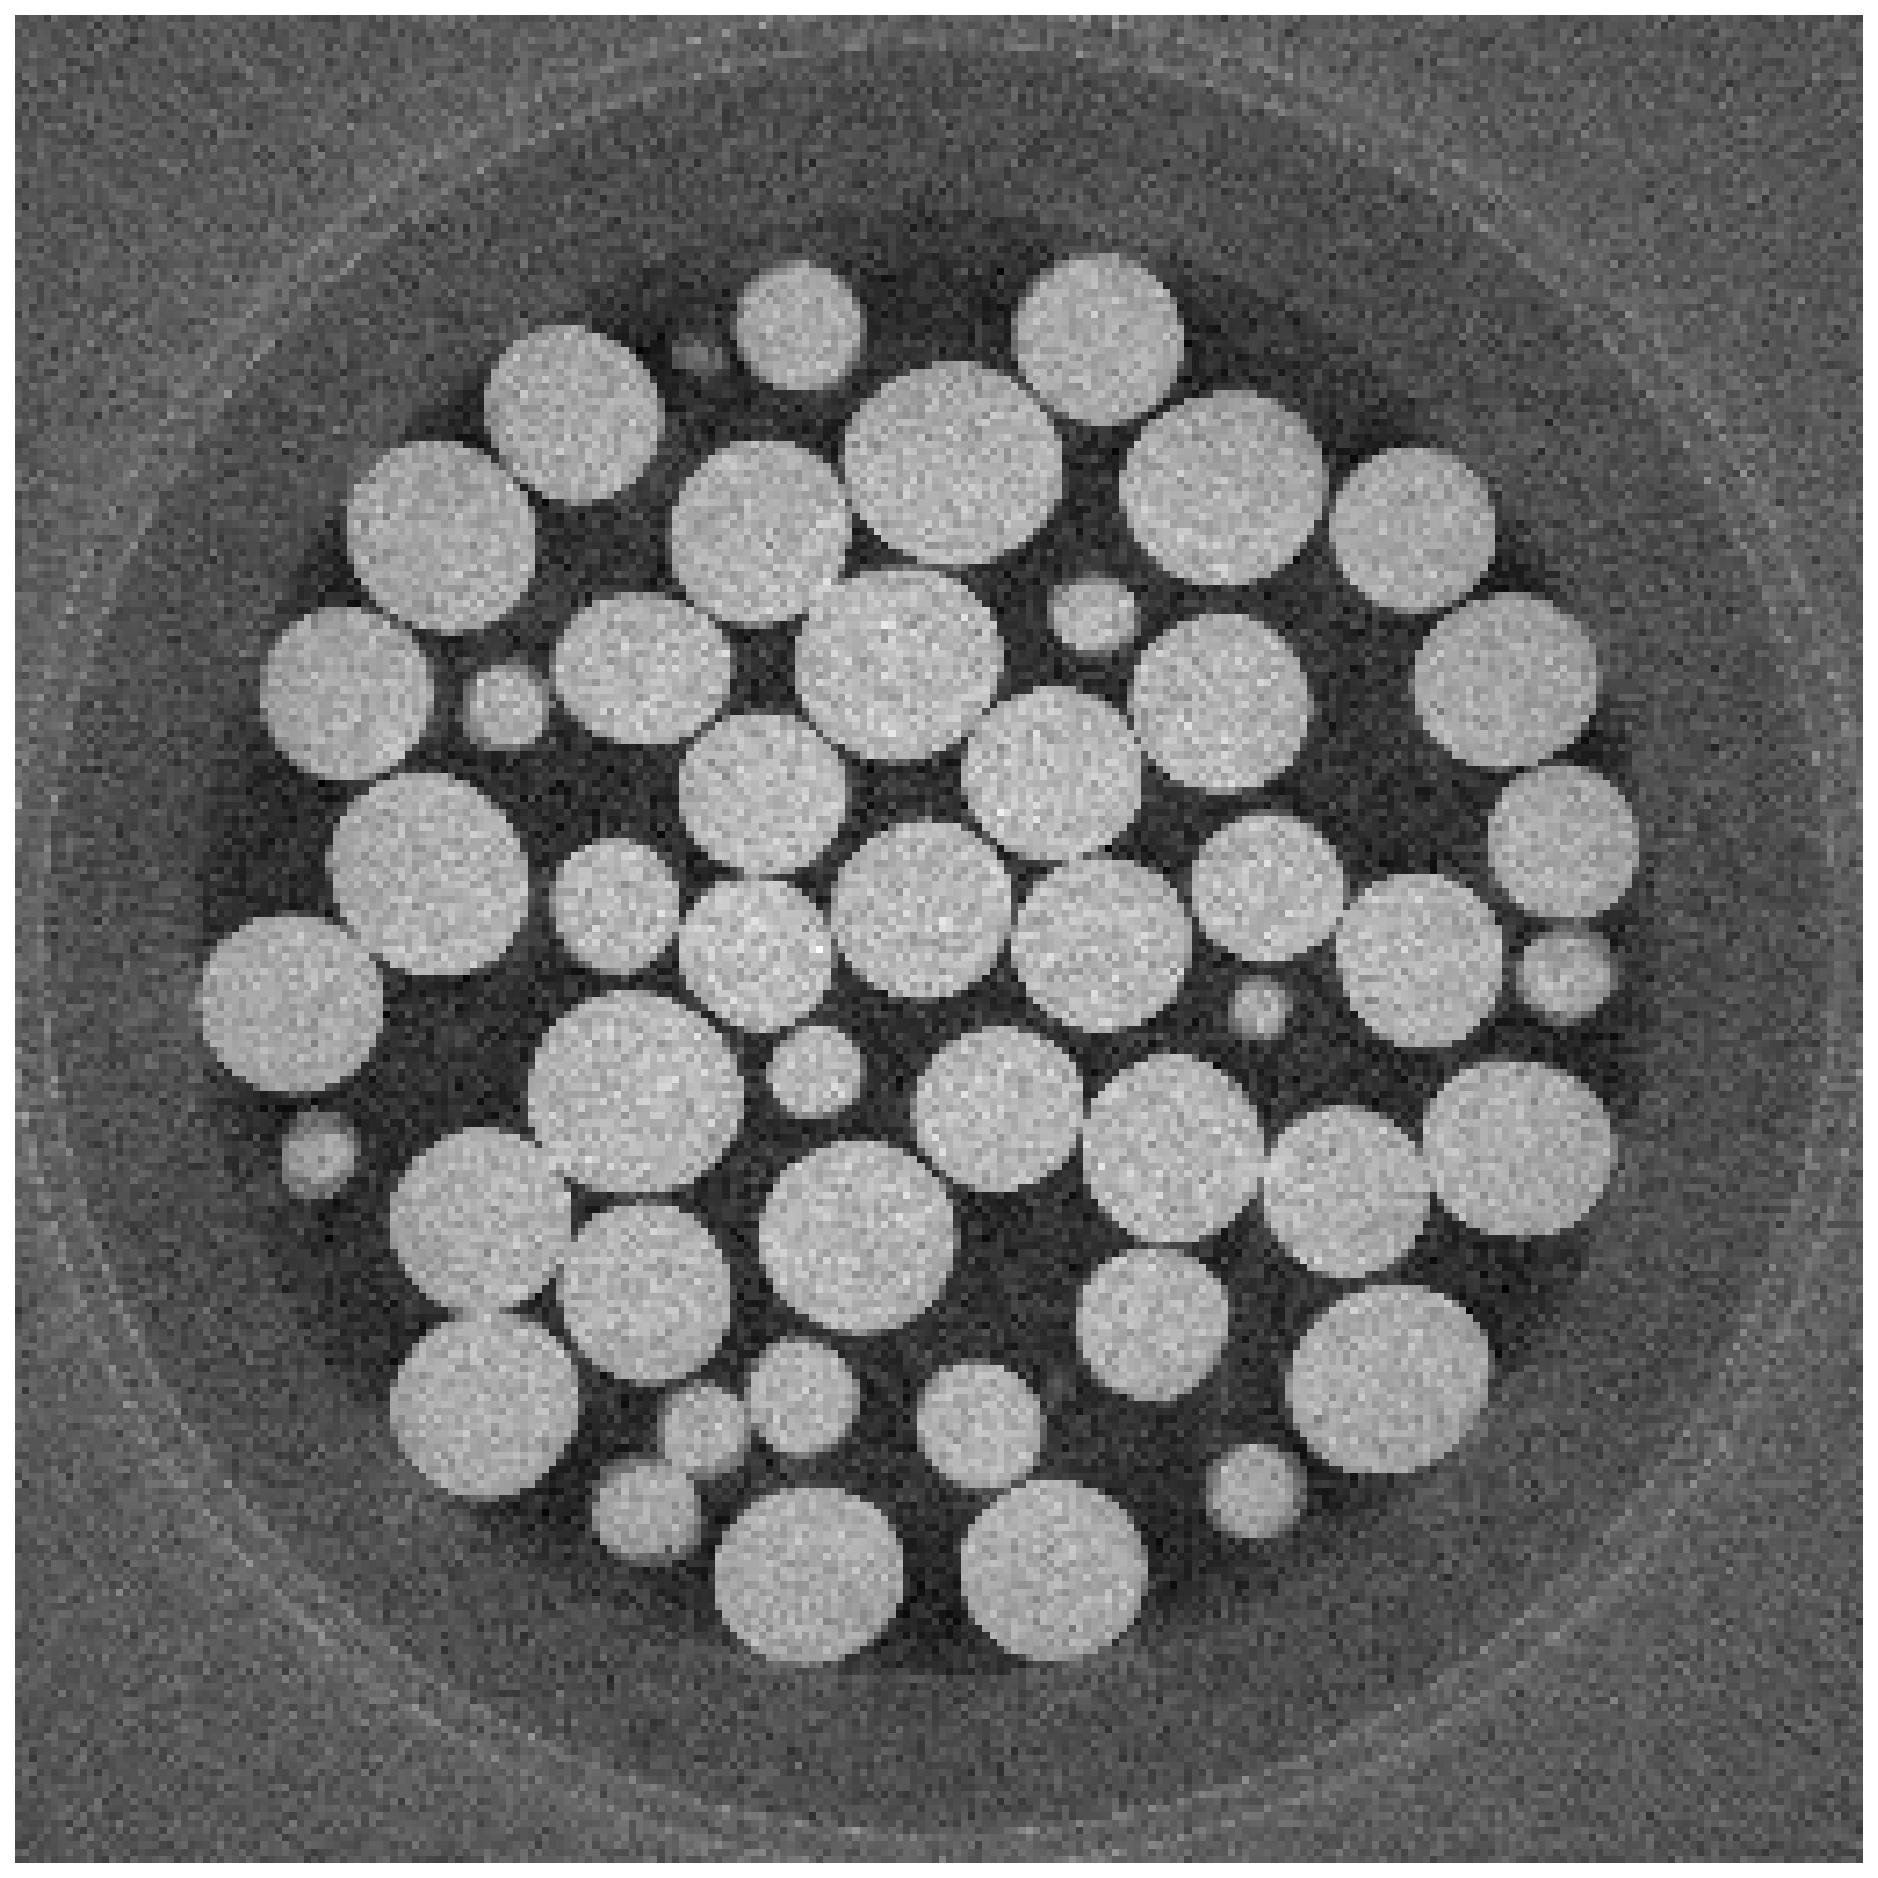
\includegraphics[width=\w\textwidth]{obj_slice.jpg}};

\node [label={[shift={(0,-2.5)}]CAD}] (CAD)[below=5mm of unknownShape.south]{
\includegraphics[width=\w\textwidth]{cad_slice.jpg} };

\node [label=Scarce sinogram] (scarceSample) [right=15mm of unknownShape.east] {\includegraphics[width=\w\textwidth]{sophia_sin_example.png}};

\node  [label={[shift={(0,-2.5)}]CAD Sinogram}] (cadSample) [below=5mm of scarceSample.south] {\includegraphics[width=\w\textwidth]{cad_sin.png}};

\node (concatenate) [right= 5mm of cadSample.east] {\scriptsize Concatenation \\ \scriptsize and \\ \scriptsize GAN inference};

\node [label={[shift={(0,-2.5)}]Inferred Sinogram}](inferred) [right= 5mm of concatenate.east] {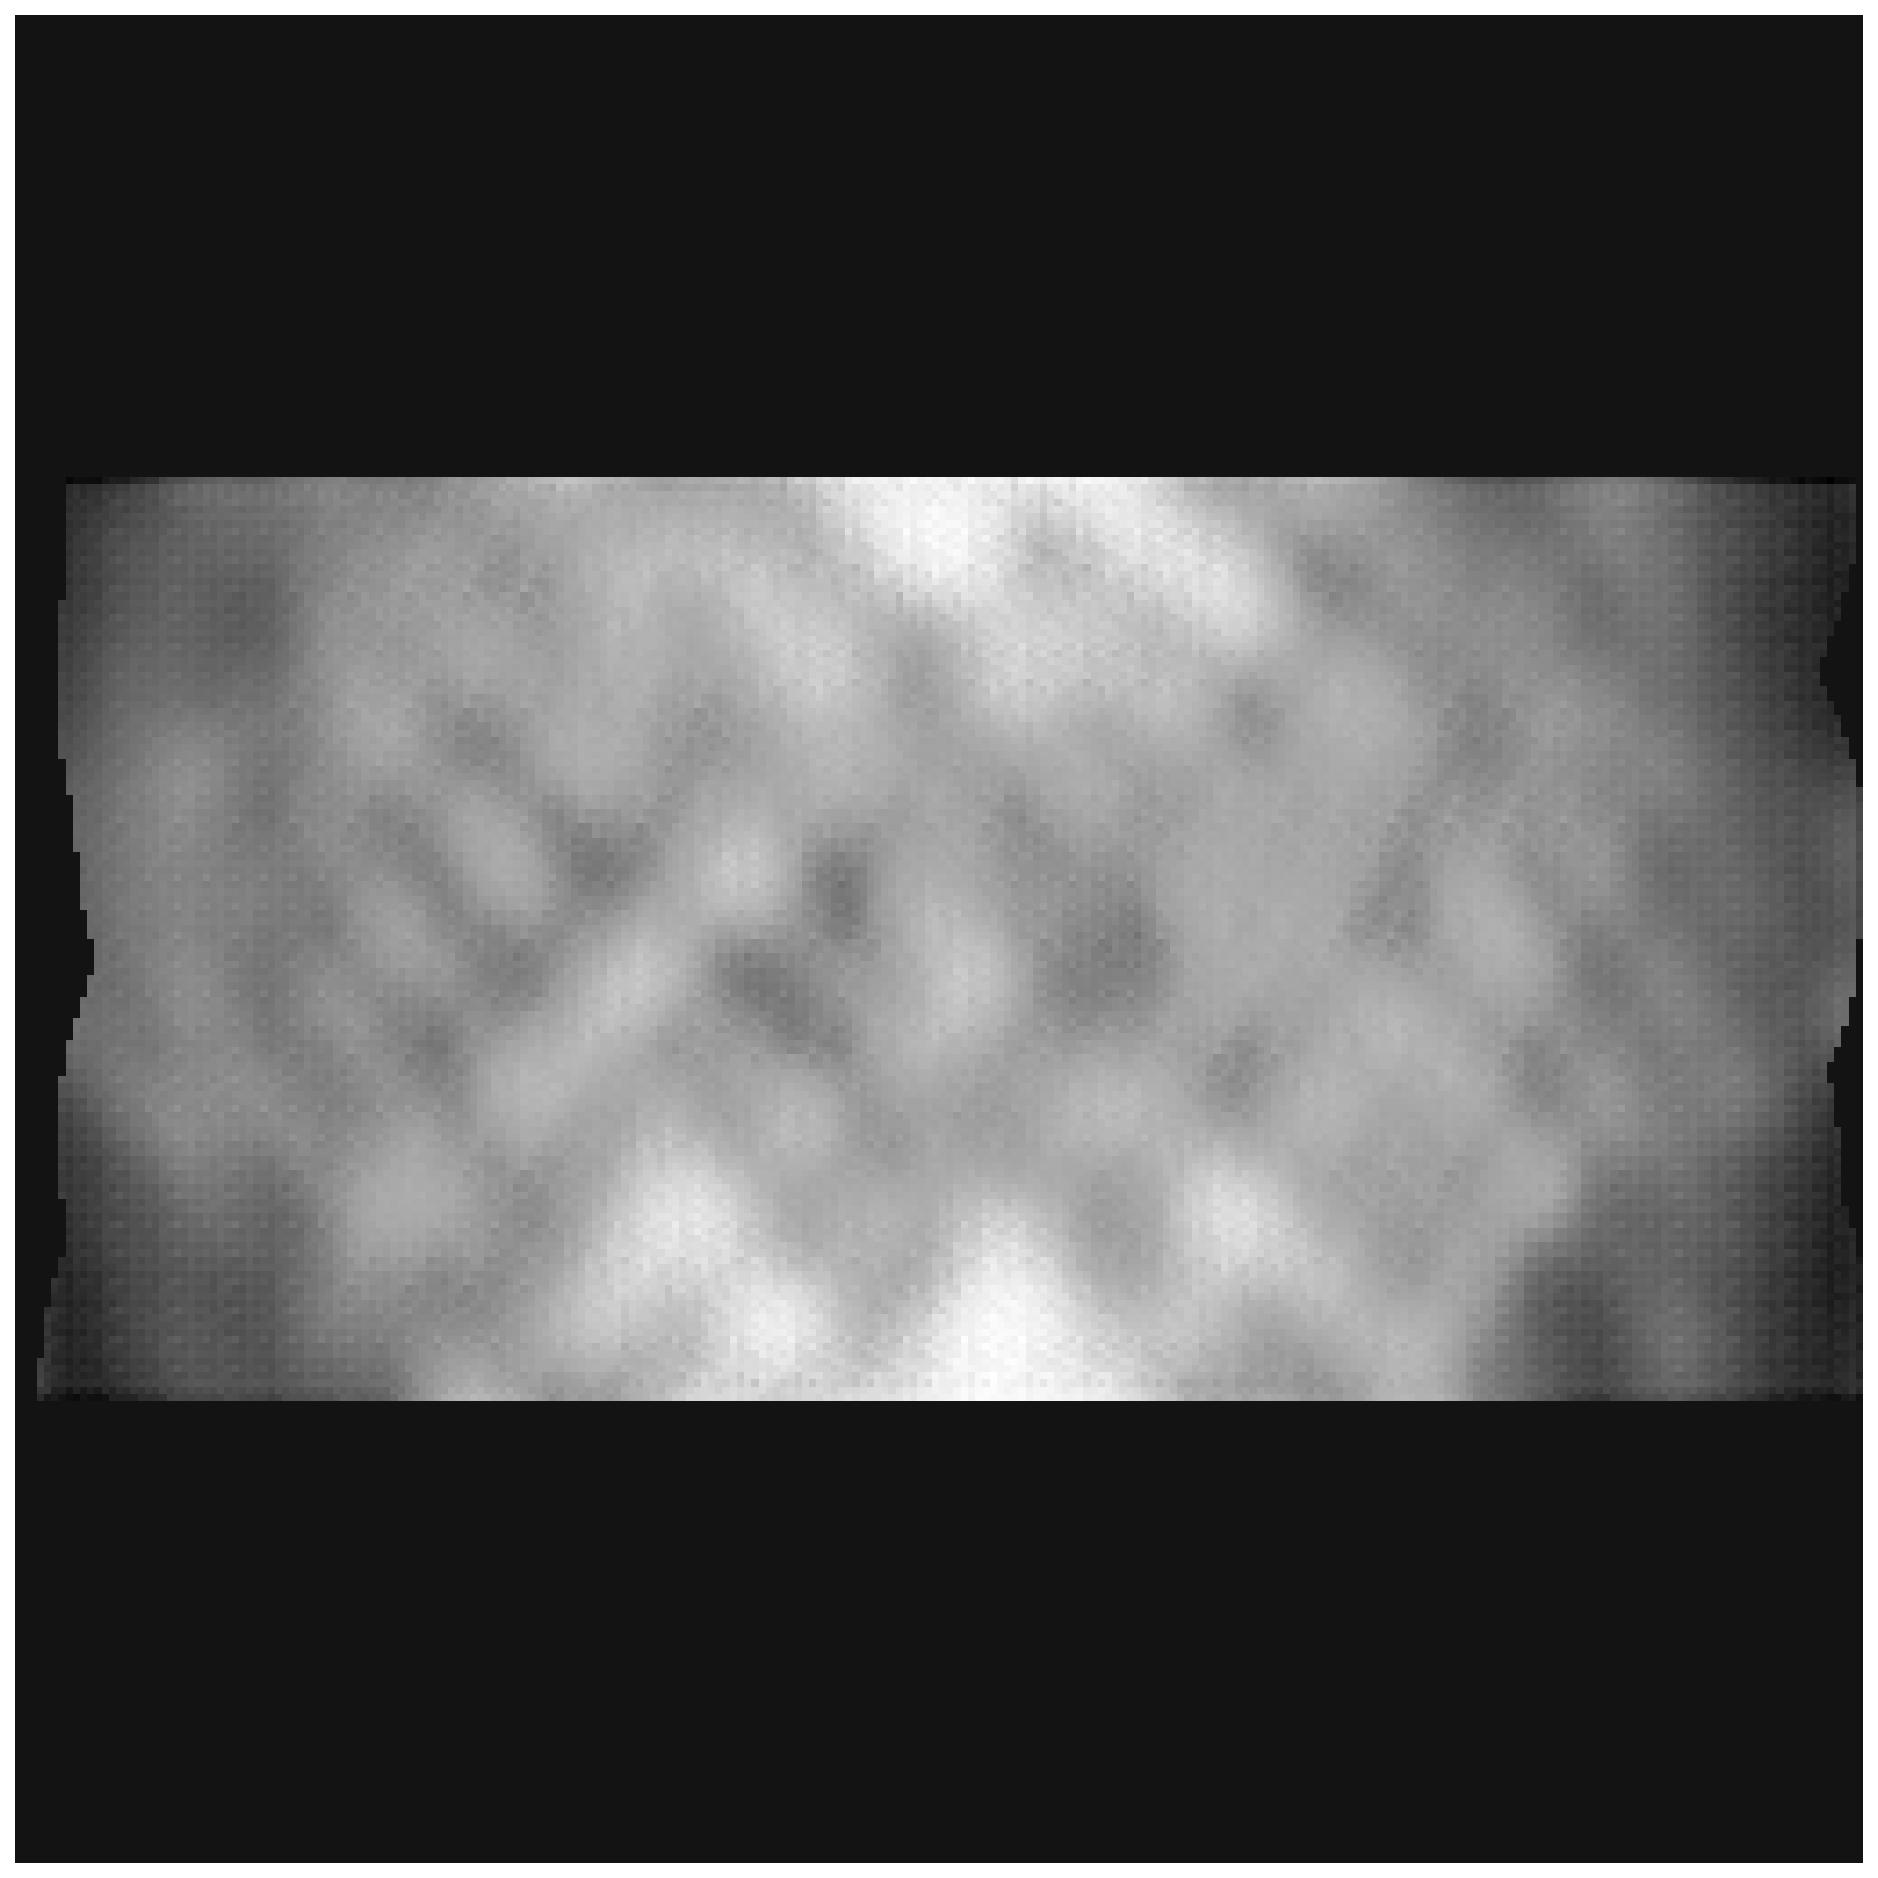
\includegraphics[width=\w\textwidth]{sinograms128_inferenceOnlyGAN.jpg}};

\node (pwAddition) [above= 10.5mm of inferred.north] {\scriptsize Pixel-wise \\ \scriptsize addition};

\node [label=Inpainted sinogram] (inpainted) [right=5mm of pwAddition.east] {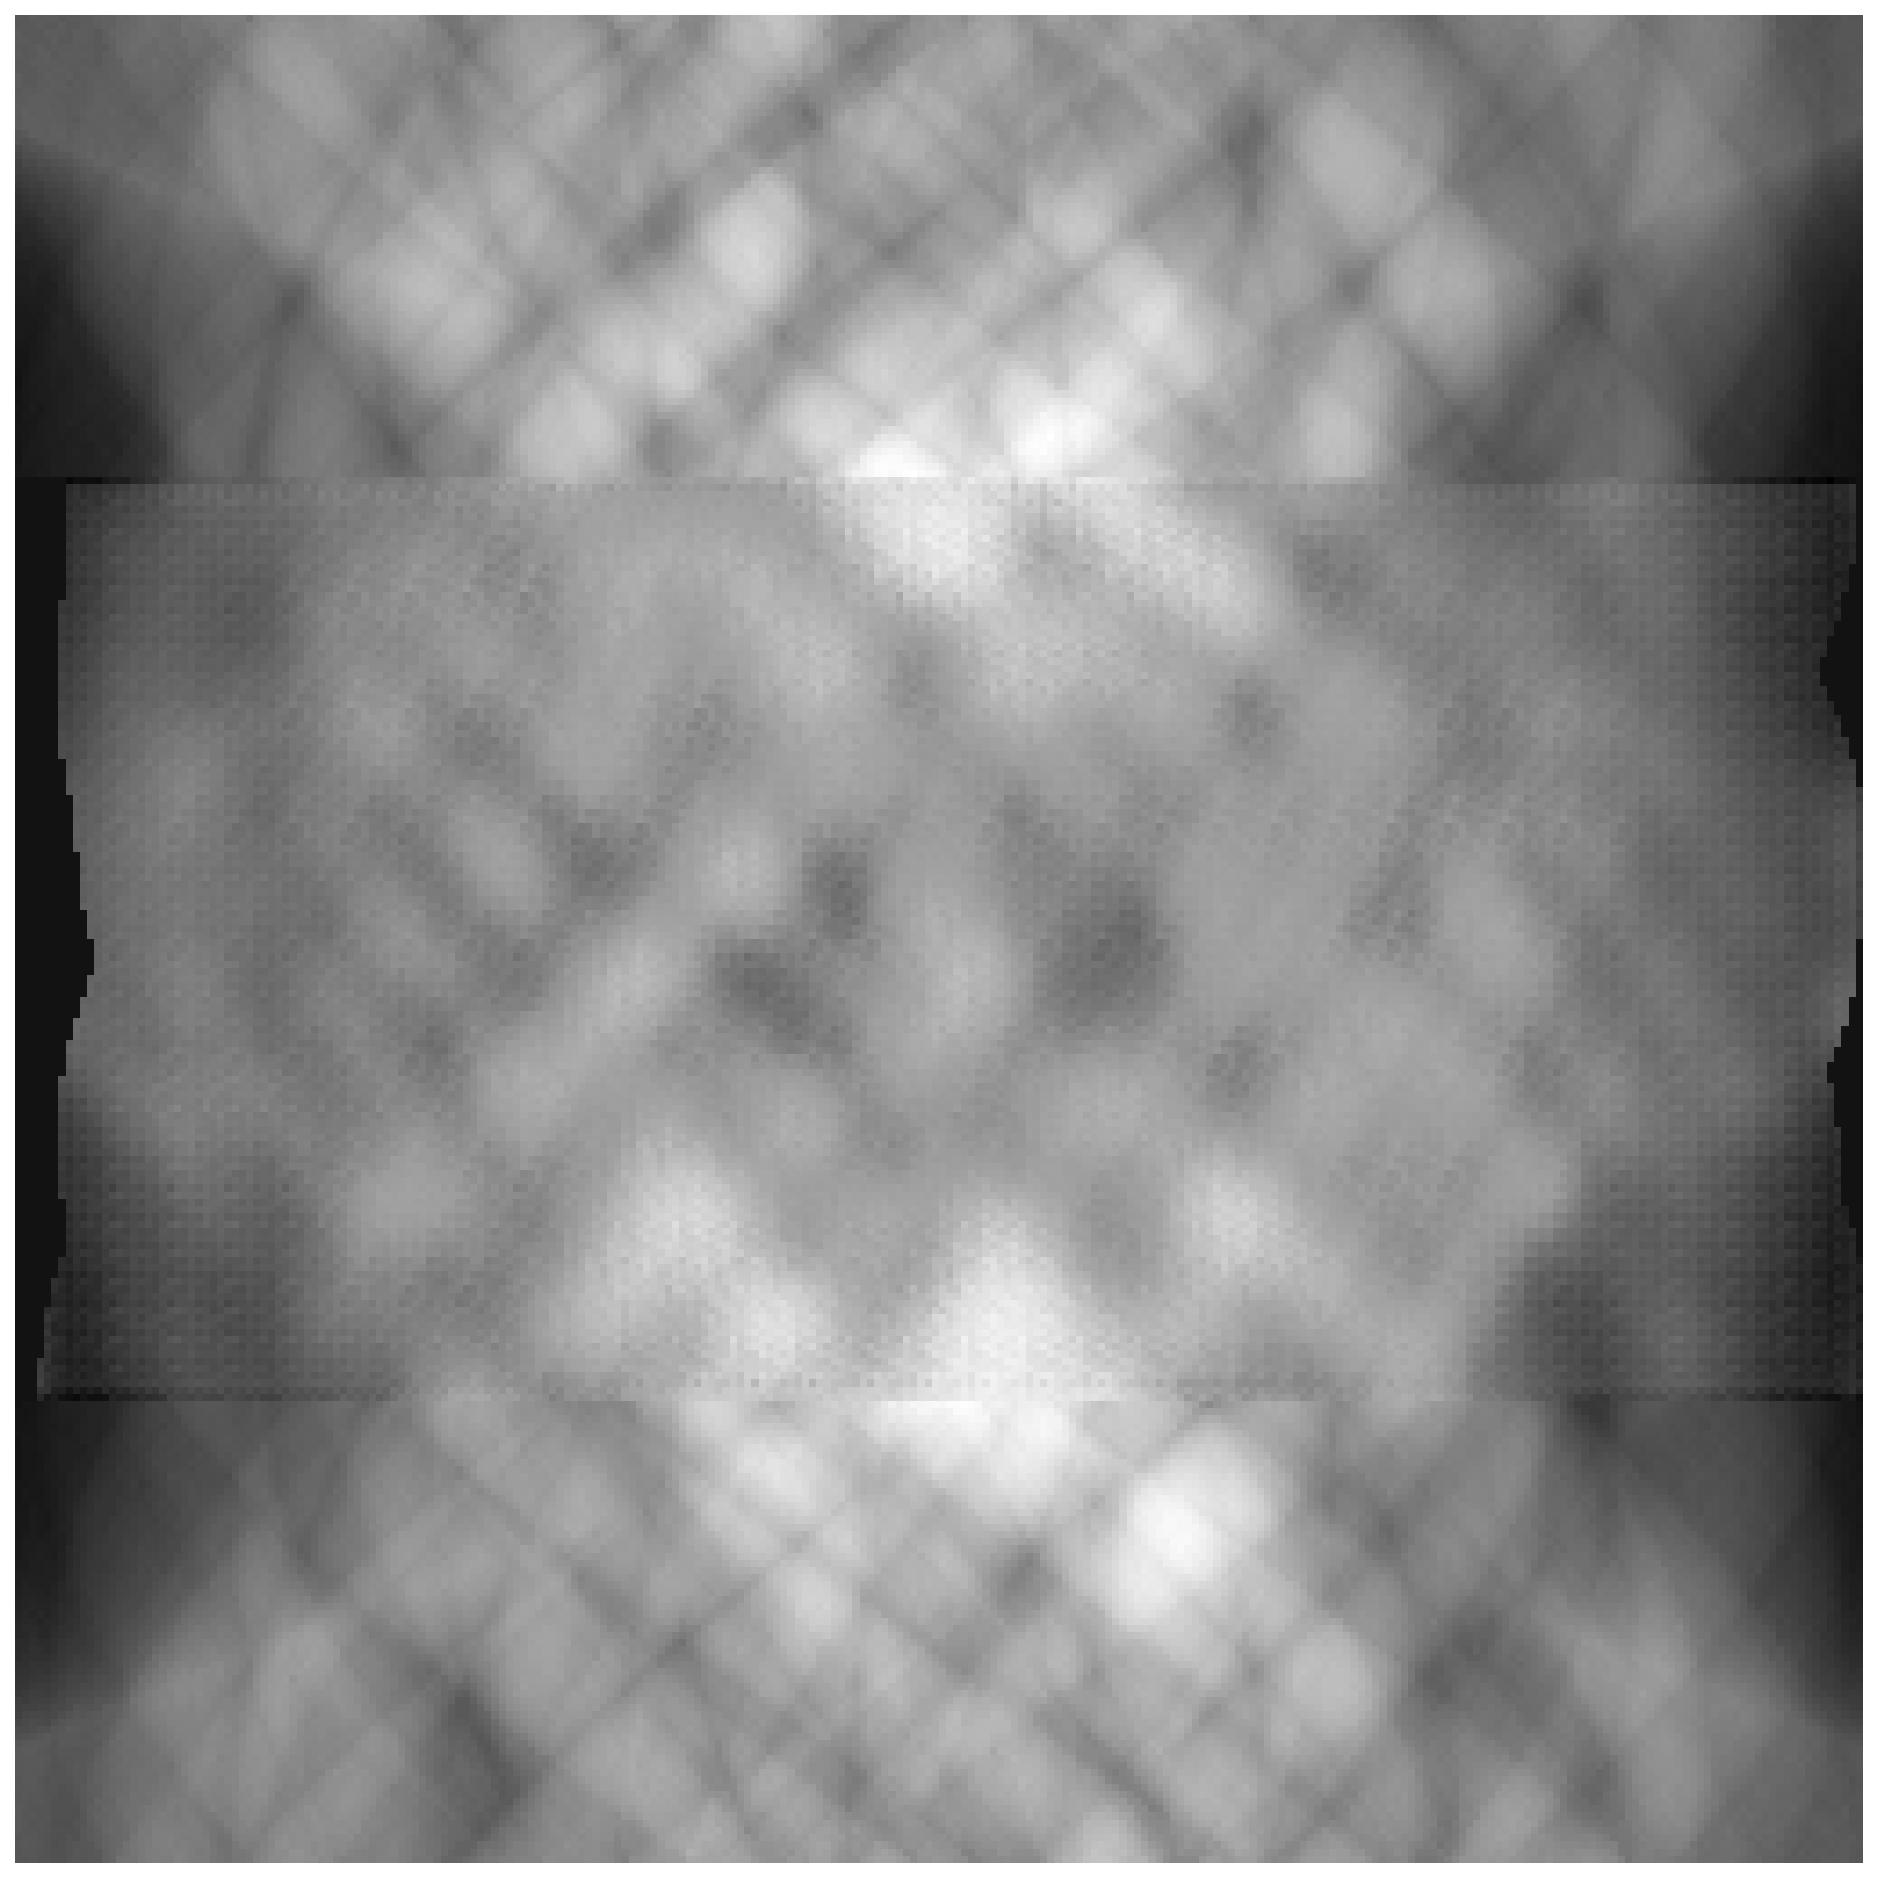
\includegraphics[width=\w\textwidth]{sinograms128_inferenceCadGan.jpg}};

\draw[->] (unknownShape) to node {\scriptsize Sampling} (scarceSample)  ;

\draw[->] (CAD) to node {\scriptsize Sampling} (cadSample) ;

\draw[->] (scarceSample.east) -- (pwAddition.west);
\draw[->] (scarceSample.east) -- (concatenate.north);

\draw[->] (cadSample) -- (concatenate);

\draw[->] (concatenate) -- (inferred) ;

\draw[->] (inferred) -- (pwAddition) ;

\draw[->] (pwAddition) -- (inpainted) ;

\end{tikzpicture}
\end{frame}
\egroup


\end{document}